\chapter[Probability Distribution Map and Task-Difficulty Map Editor Interface]{Probability Distribution Map and Task-Difficulty Map Editor Interface}
\label{chap:MapEdit}

At the \textbf{Between-Episodes} scale, a searcher might have additional case-specific information (e.g, past experience, knowledge of the search area or weather conditions, or the profile of the missing person) and would like to modify the general plan produced at the strategic scale. Moreover, as search progresses, the search plan should change due to newly found evidence (or the lack of it) from either the ground searchers or previous UAV flights. We developed two autonomy management tools at this scale that allow the user to manage two types of information: \textit{probability distribution map} and \textit{task-difficulty map}.

\begin{figure}
\centering
\begin{tabular}{cc}
	\begin{minipage}{0.45\textwidth}
	\centering
	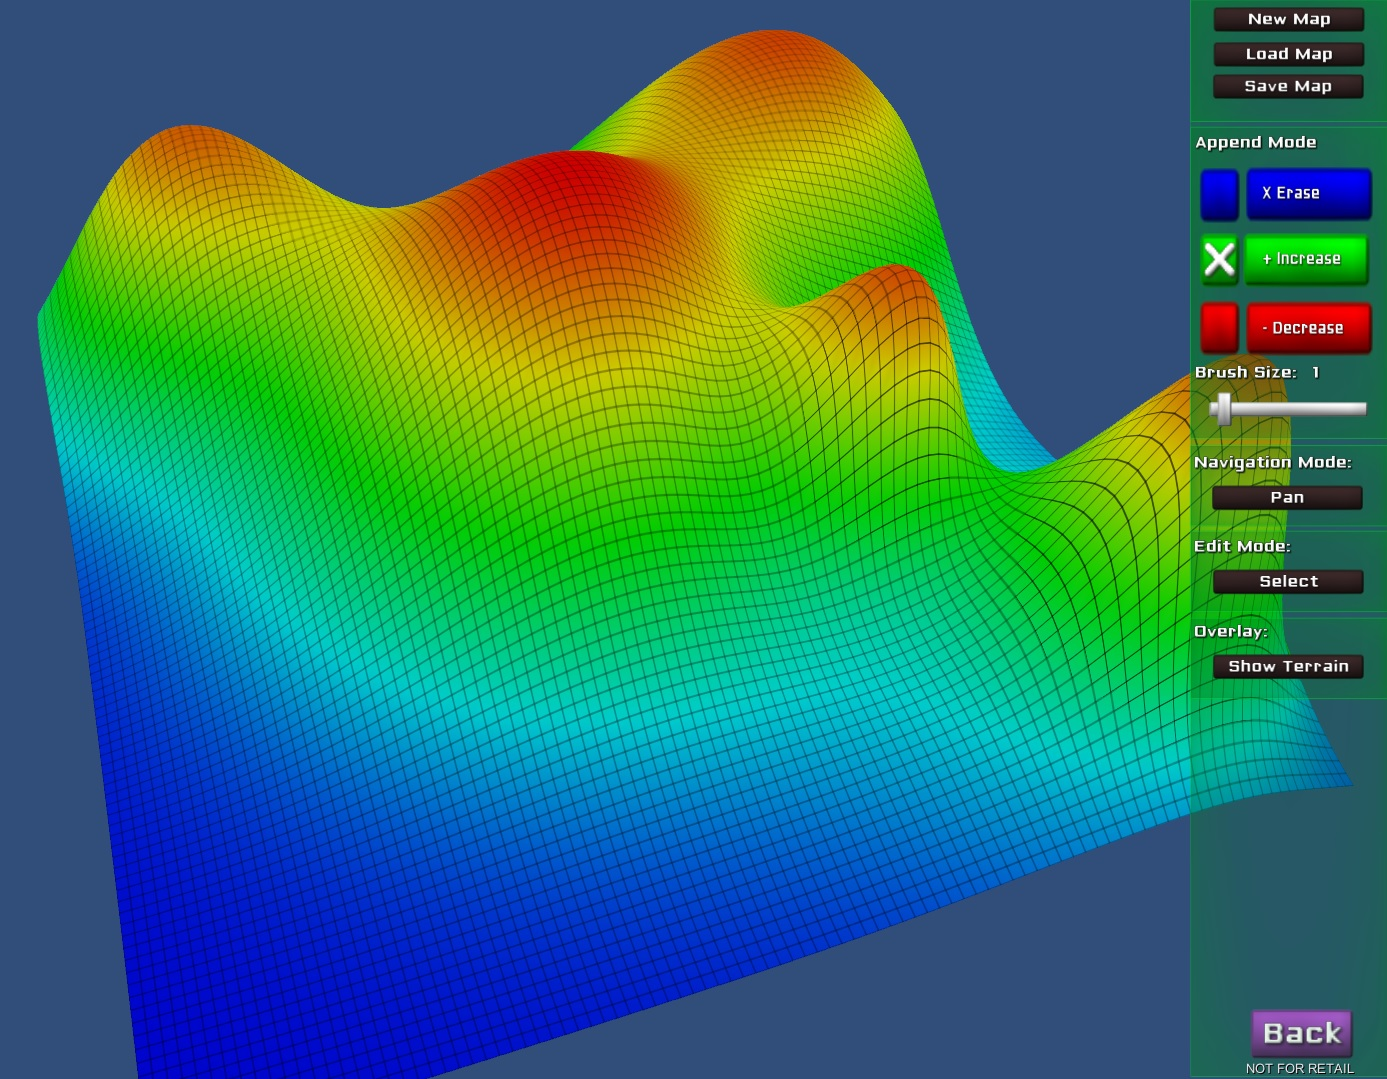
\includegraphics[width=2.8in]{DistEditExample.jpg}
	\caption{An example probability distribution map generated using the DistEdit tool.}
	\label{DistEditExample2}
	\end{minipage}
&
	\begin{minipage}{0.45\textwidth}
	\centering
	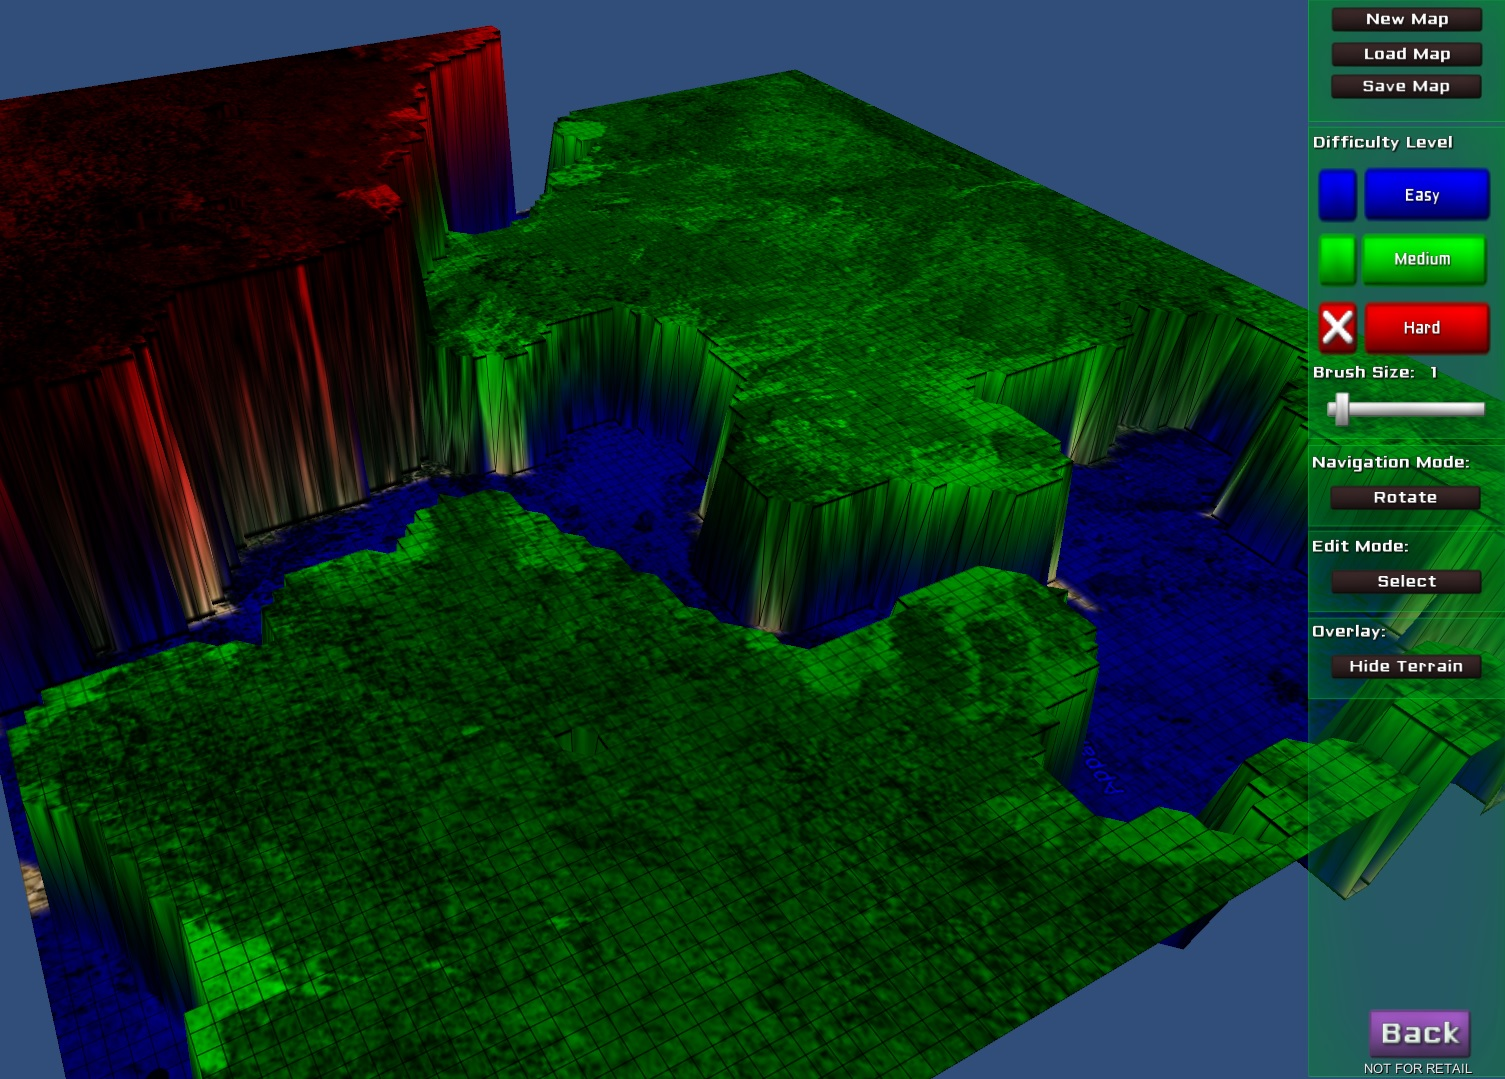
\includegraphics[width=2.8in]{DiffEditExample.jpg}
	\caption{An example task-difficulty map generated using the DiffEdit tool with satellite image of the search region overlaid on top.}
	\label{DiffEditExample2}
	\end{minipage}
\end{tabular}
\end{figure}

Searchers can use the \textbf{DistEdit} tool to modify a probability distribution map and use the \textbf{DiffEdit} tool to modify a task-difficulty map generated at the \textbf{Strategic} scale. Both tools enable the user to view maps as 3D surfaces where a color map is applied for better distinction (red means high probability area or high task-difficulty level and blue means low vise versa). The user can use mouse and finger gestures to rotate/pan/zoom the respective map and edit the shapes of the maps in 3D to incorporate information that the autonomous components are unable to interpret. The user also has the option to overlay a satellite image of the search area on top of the maps for better alignments and precision.

If the user is dissatisfied with the \textit{probability distribution map} or \textit{task-difficulty map} systematically generated at the \textbf{Strategic} scale, using the \textbf{DistEdit} and \textbf{DiffEdit} tools he or she can also create a \textit{probability distribution map} and/or a \textit{task-difficulty map} from scratch. Figure~\ref{DistEditExample2} and~\ref{DiffEditExample2} show screen captures of these two tools and also example maps generated using the two tools.

Both tools enable the searchers to incoporate additional information only the user can process into information representations the autonomous components of the UAV system can understand, and then rely on UAV path-planning to use the information to search more efficiently.

%=====================================================================================================
\section{The DiffEdit Tool}
\label{DiffEdit}

The \textbf{DiffEdit} enables the user to create or modify a \textit{task-difficulty map} by marking areas with different levels of difficulty. When using a UAV to support Wilderness Search and Rescue (WiSAR), task difficulty is related to sensor detection probability. A difficult area on the map represents places where the probability of detecting the missing person is low (maybe due to terrain features, vegetation density, or lighting conditions). By marking an area with high task difficulty, the user can indirectly tell the UAV to make multiple passes in the area, or avoid the area and set high priority to areas marked with low task difficulty. When combined with a \textif{probability distribution map}, an area with medium probability and low task difficulty may be more attractive than an area with high probability but high task difficulty.

%===================================================
\subsection{Editing vs. Starting New}


%===================================================
\subsection{3D Navigation Controls}

Inside the \textbf{DiffEdit} tool the \textif{task-difficulty map} is shown as a 3D surface, and task difficulty is represented by both height and color. Areas with low height in blue represents areas in the search region with 


%===================================================
\subsection{Task Difficulty Levels}

The tool currently supports three difficulty levels (easy, medium, and hard) but can be easily extended to support more difficulty levels. The \textbf{DiffCreate} component at the \textbf{Strategic} level can automatically create a \textif{task-difficulty map} based on vegetation density information extrapolated from USGS satellite imageries. The user can choose to load this systematically generated \textif{task-difficulty map} into the \textbf{DiffEdit} tool and then make modifications using mouse or finger gestures. Figure~\ref{DiffEdit003} shows such a \textif{task-difficulty map} generated by the \textbf{DiffCreate} component with modifications made using the \textbf{DiffEdit} tool (circular shapes at the left side of the figure). 


%===================================================
\subsection{Painting Mode vs. Lasso Select Mode}


In \textbf{DiffEdit} the user can specify \textit{task difficulty} by using a paintbrush tool to paint on the task-difficulty map with scribbles. The user can also use a lasso tool to specify a region of irregular shape and then mark the region with selected task-difficulty level. By marking an area as a difficult area, the user can indirectly tell the UAV to make multiple passes over these areas to search more thoroughly. Figure~\ref{DiffEditExample2} shows an example task-difficulty map generated using the \textbf{DiffEdit} tool with the satellite image of the search region overlaid on top.



\textif{task-difficulty map}
\textif{task-difficulty map}
\textif{task-difficulty map}
\textif{task-difficulty map}
\textif{task-difficulty map}
\textif{task-difficulty map}


\textbf{DiffEdit}
\textbf{DiffEdit}
\textbf{DiffEdit}
\textbf{DiffEdit}




\begin{figure}
\centering
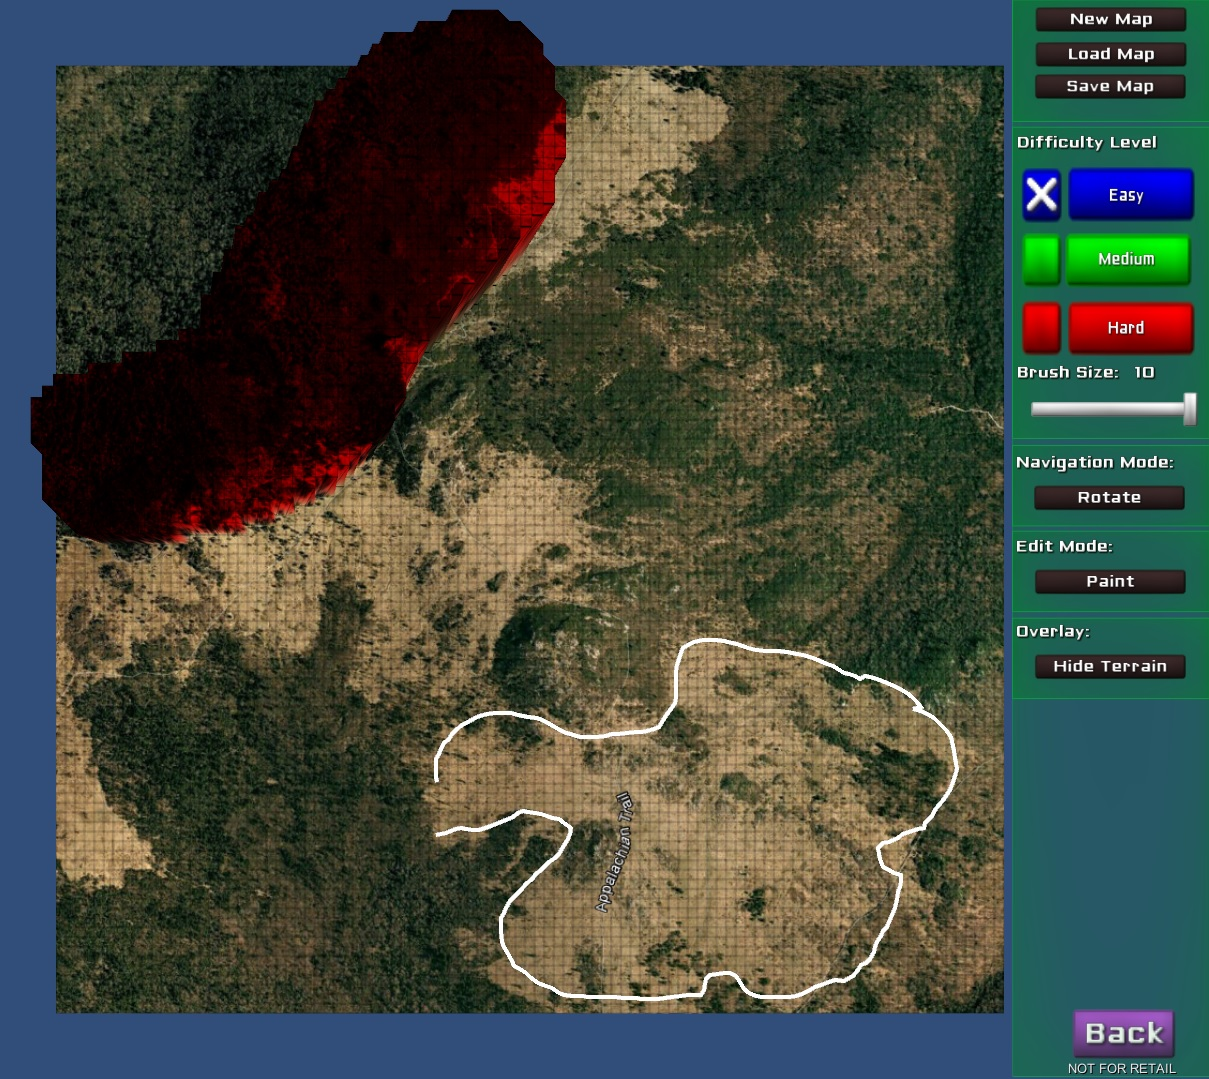
\includegraphics[width=6in]{DiffEdit001.JPG}
\caption{To be added}
\label{DiffEdit001}
\end{figure}

\begin{figure}
\centering
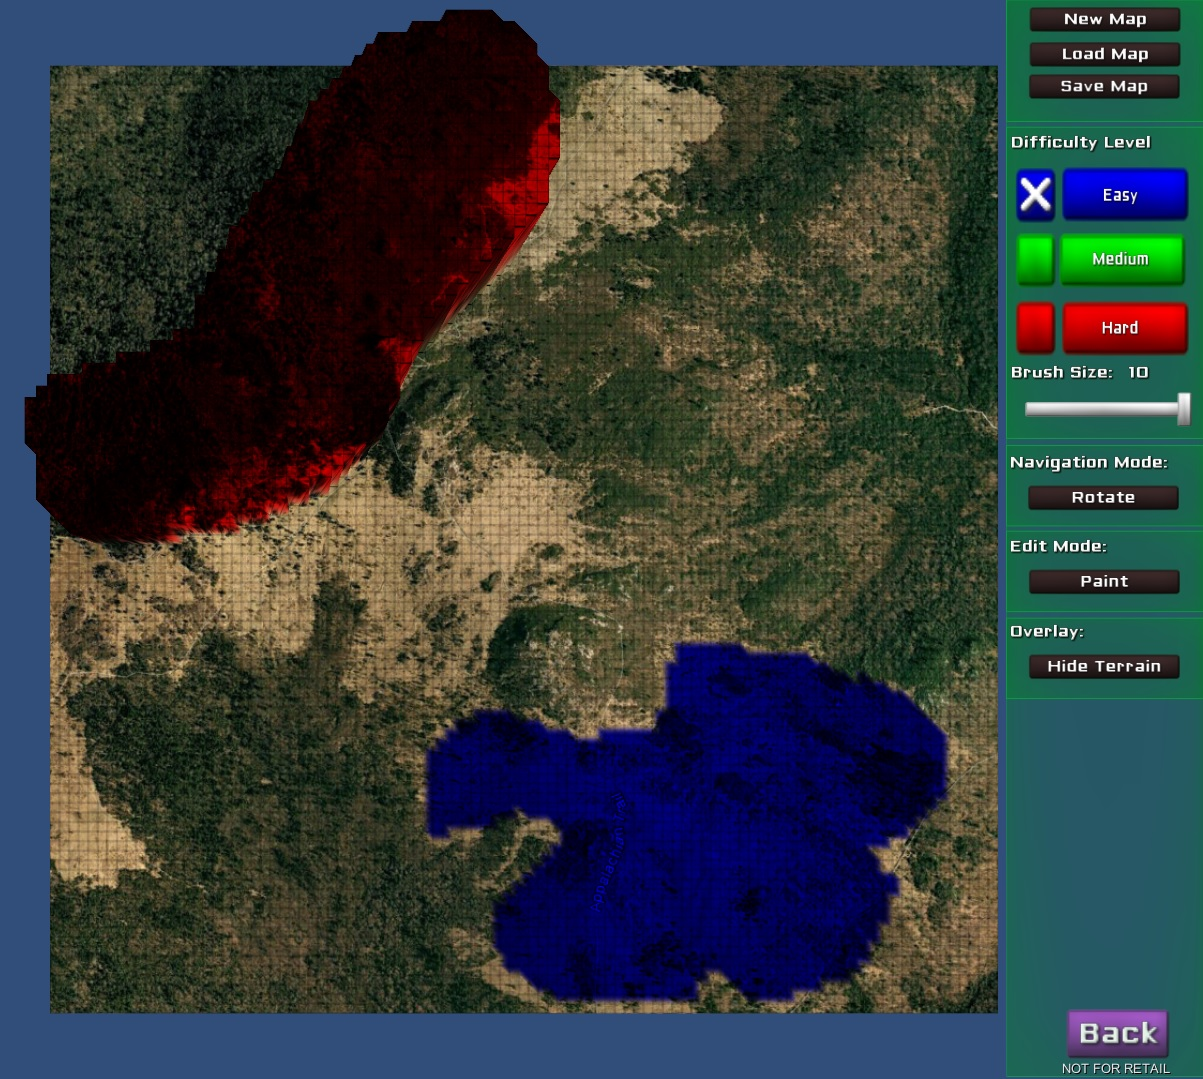
\includegraphics[width=6in]{DiffEdit002.JPG}
\caption{To be added}
\label{DiffEdit002}
\end{figure}

\begin{figure}
\centering
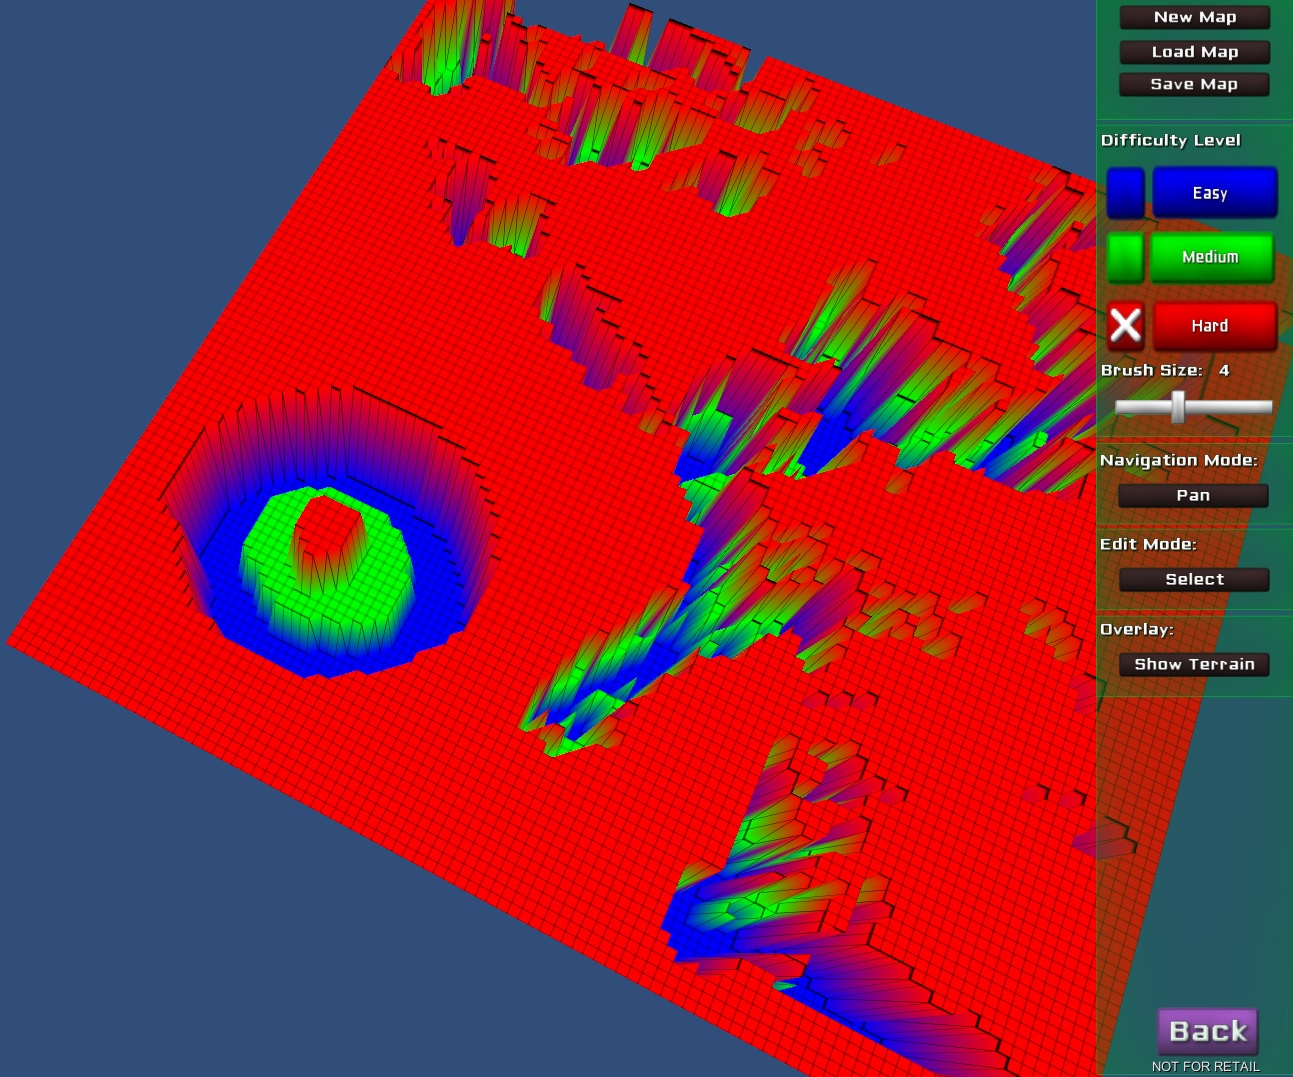
\includegraphics[width=6in]{DiffEdit003.JPG}
\caption{To be added}
\label{DiffEdit003}
\end{figure}


%=====================================================================================================
\section{The DistEdit Tool}
\label{DistEdit}


%===================================================
\subsection{Editing vs. Starting New}


%===================================================
\subsection{3D Navigation Controls}


%===================================================
\subsection{Task Difficulty Levels}


%===================================================
\subsection{Painting Mode vs. Lasso Select Mode}










In \textbf{DistEdit} the user can paint Gaussian distributions onto the probability distribution map (in the form of a 3D surface) with a paintbrush tool to specify \textit{areas of focus}. The mouse click (or finger press gesture) position determines the mean of the Gaussian distribution; brush size determines the standard deviation (with a radius equivalent to three times the standard deviation); and the duration of the click (or finger press gesture) determines the scale of the Gaussian distribution. Using this tool the user can add or subtract Gaussian components to the map to create a mixture of Gaussians. The modified probability distribution can be used later to prioritize tasks and plan UAV paths. By marking an area as a high priority area, the searchers can indirectly manipulate the UAV to search the area before other areas without the need to manually specify waypoints. Figure~\ref{DistEditExample2} shows an example probability distribution map generated using the \textbf{DistEdit} tool.


\begin{figure}
\centering
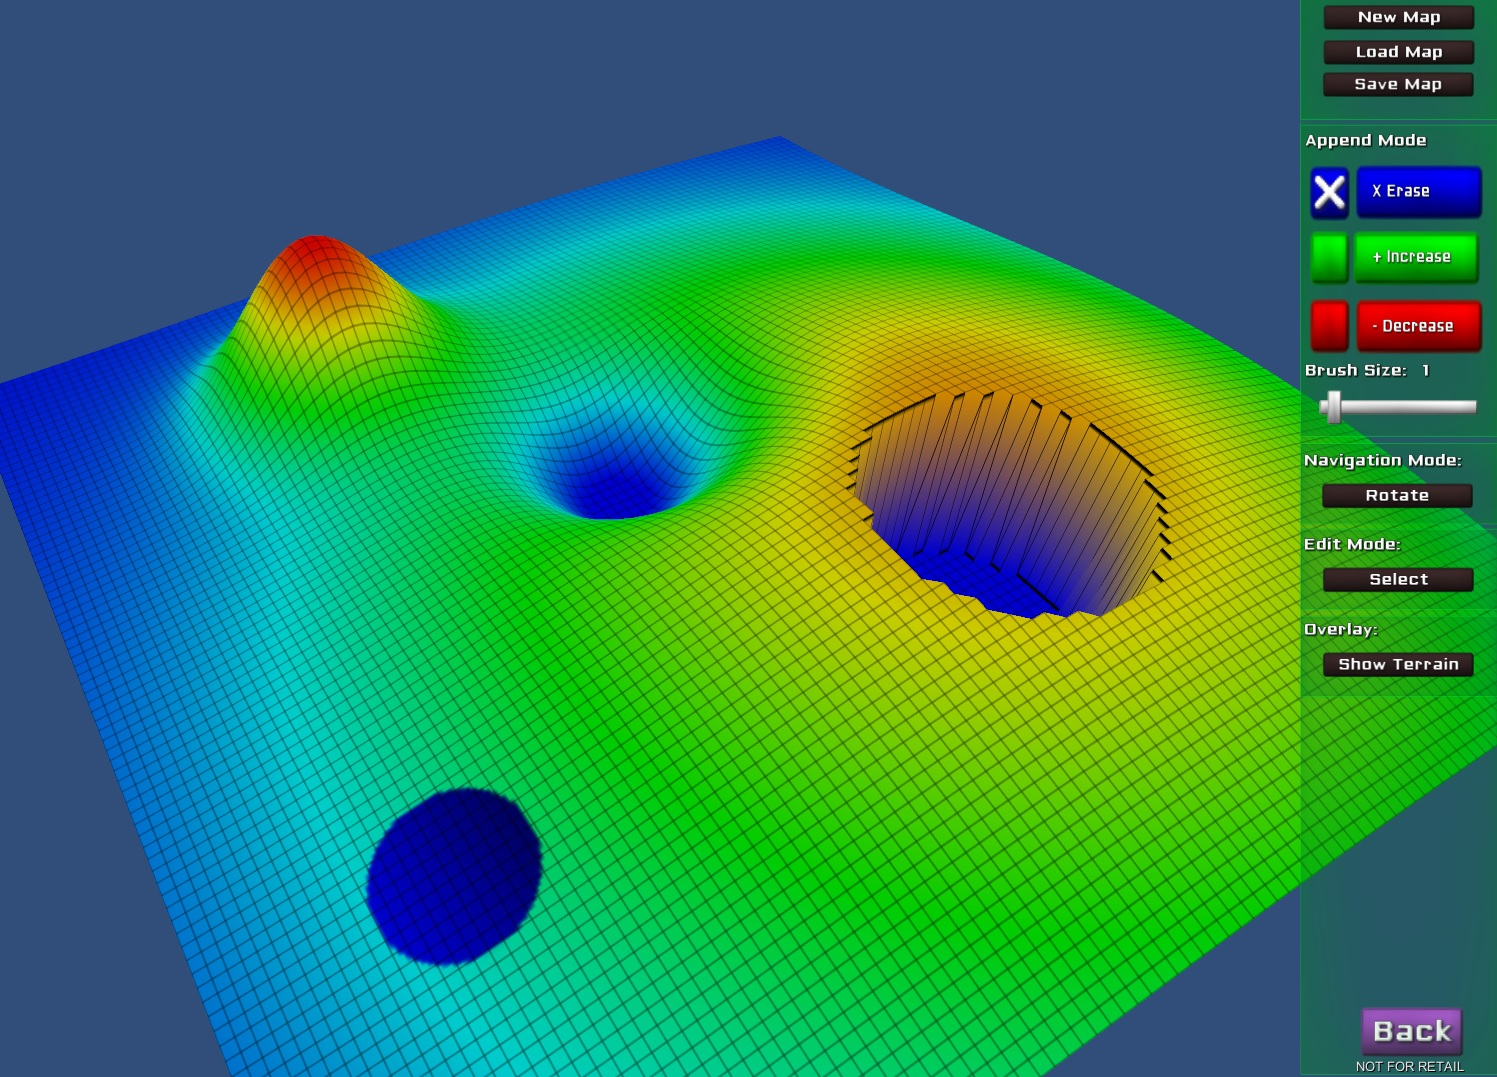
\includegraphics[width=6in]{DistEdit001.JPG}
\caption{To be added}
\label{DistEdit001}
\end{figure}

\begin{figure}
\centering
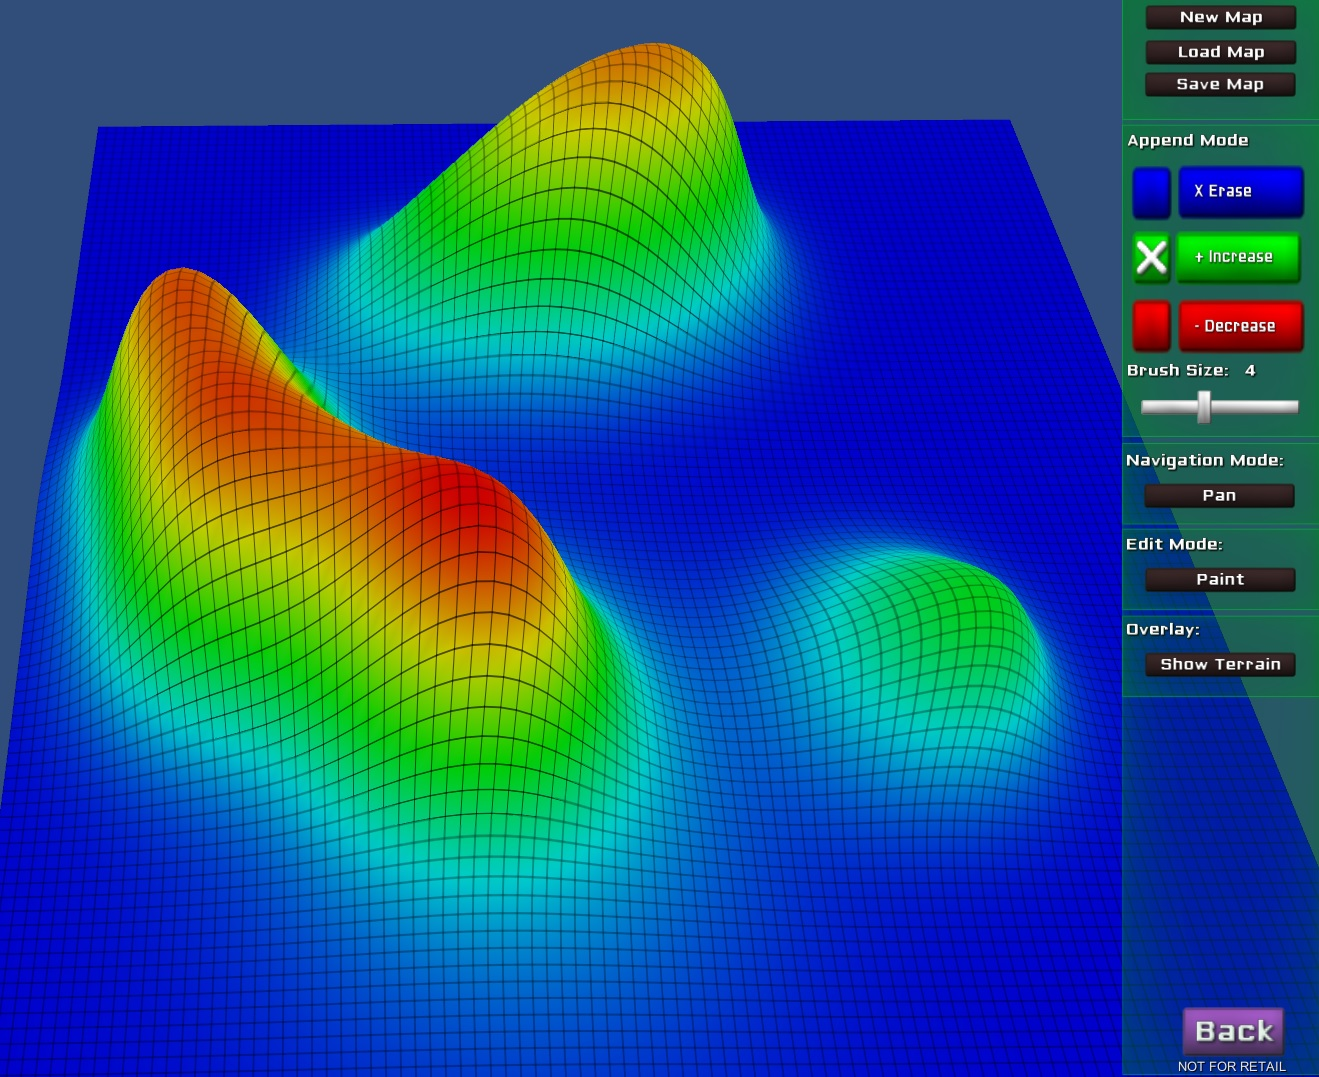
\includegraphics[width=6in]{DistEdit002.JPG}
\caption{To be added}
\label{DistEdit002}
\end{figure}

\begin{figure}
\centering
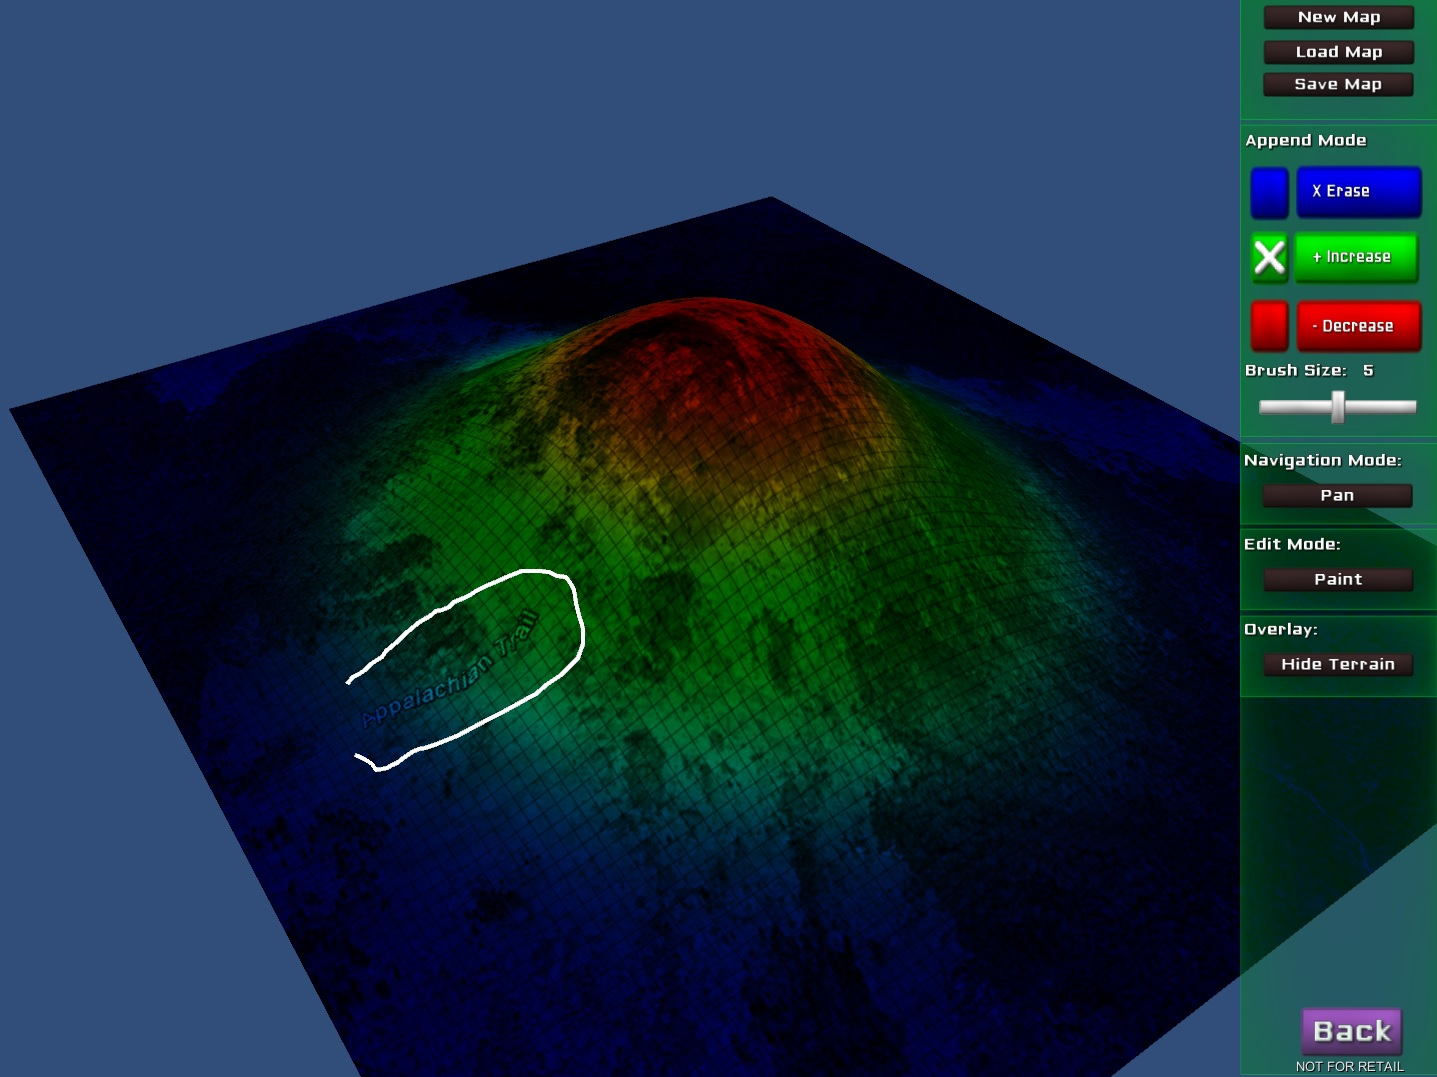
\includegraphics[width=6in]{DistEdit003.JPG}
\caption{To be added}
\label{DistEdit003}
\end{figure}

\begin{figure}
\centering
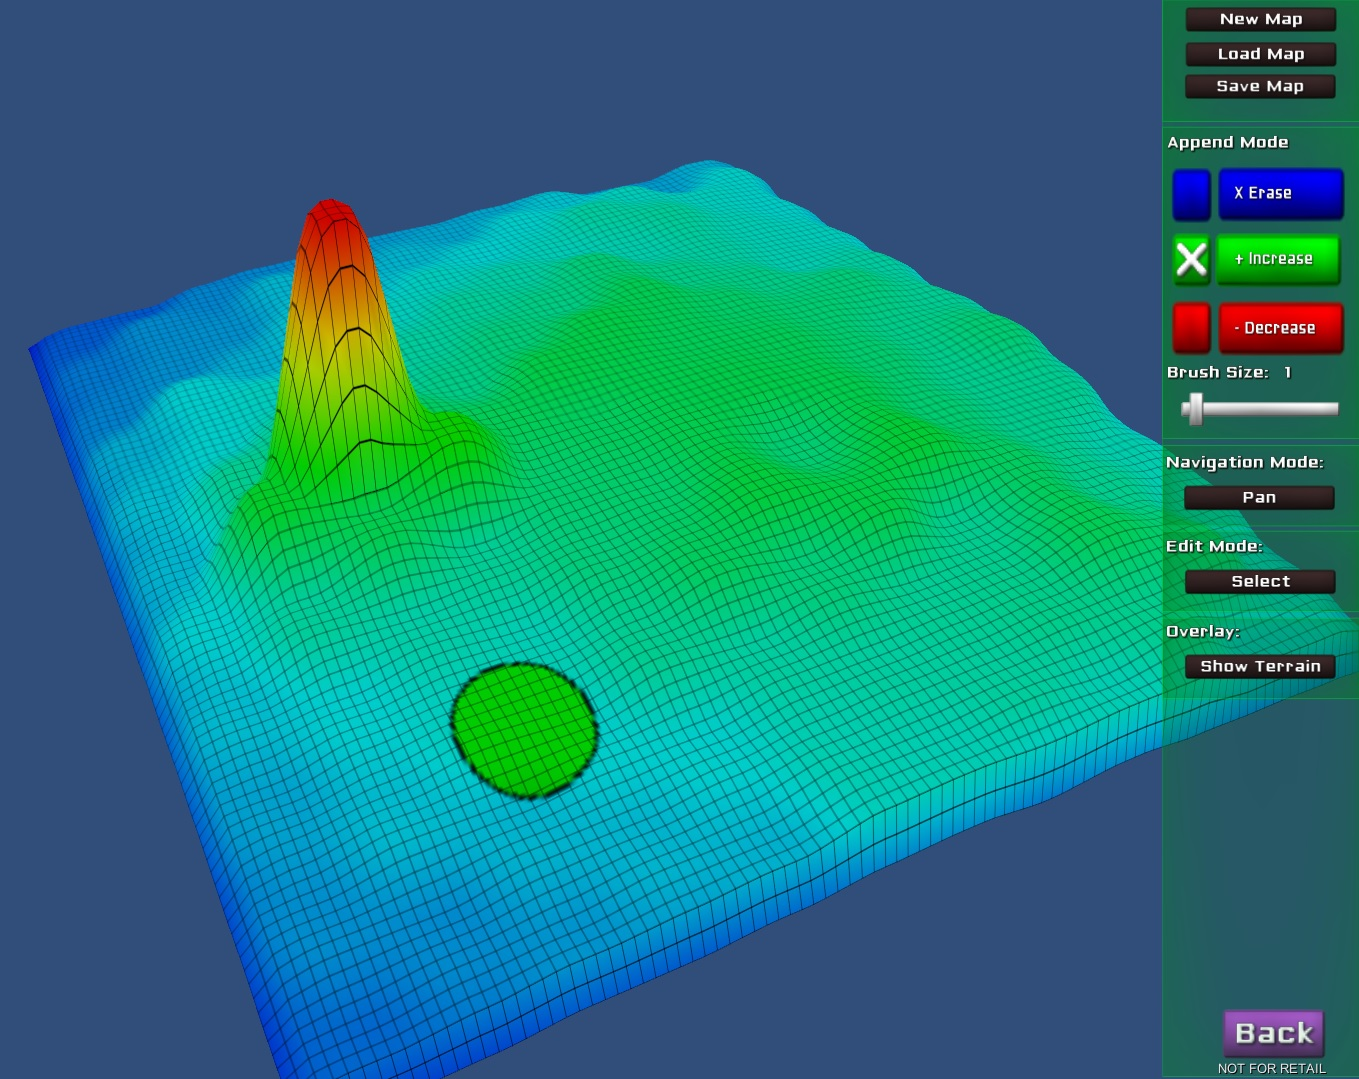
\includegraphics[width=6in]{DistEdit004.JPG}
\caption{To be added}
\label{DistEdit004}
\end{figure}

\begin{figure}
\centering
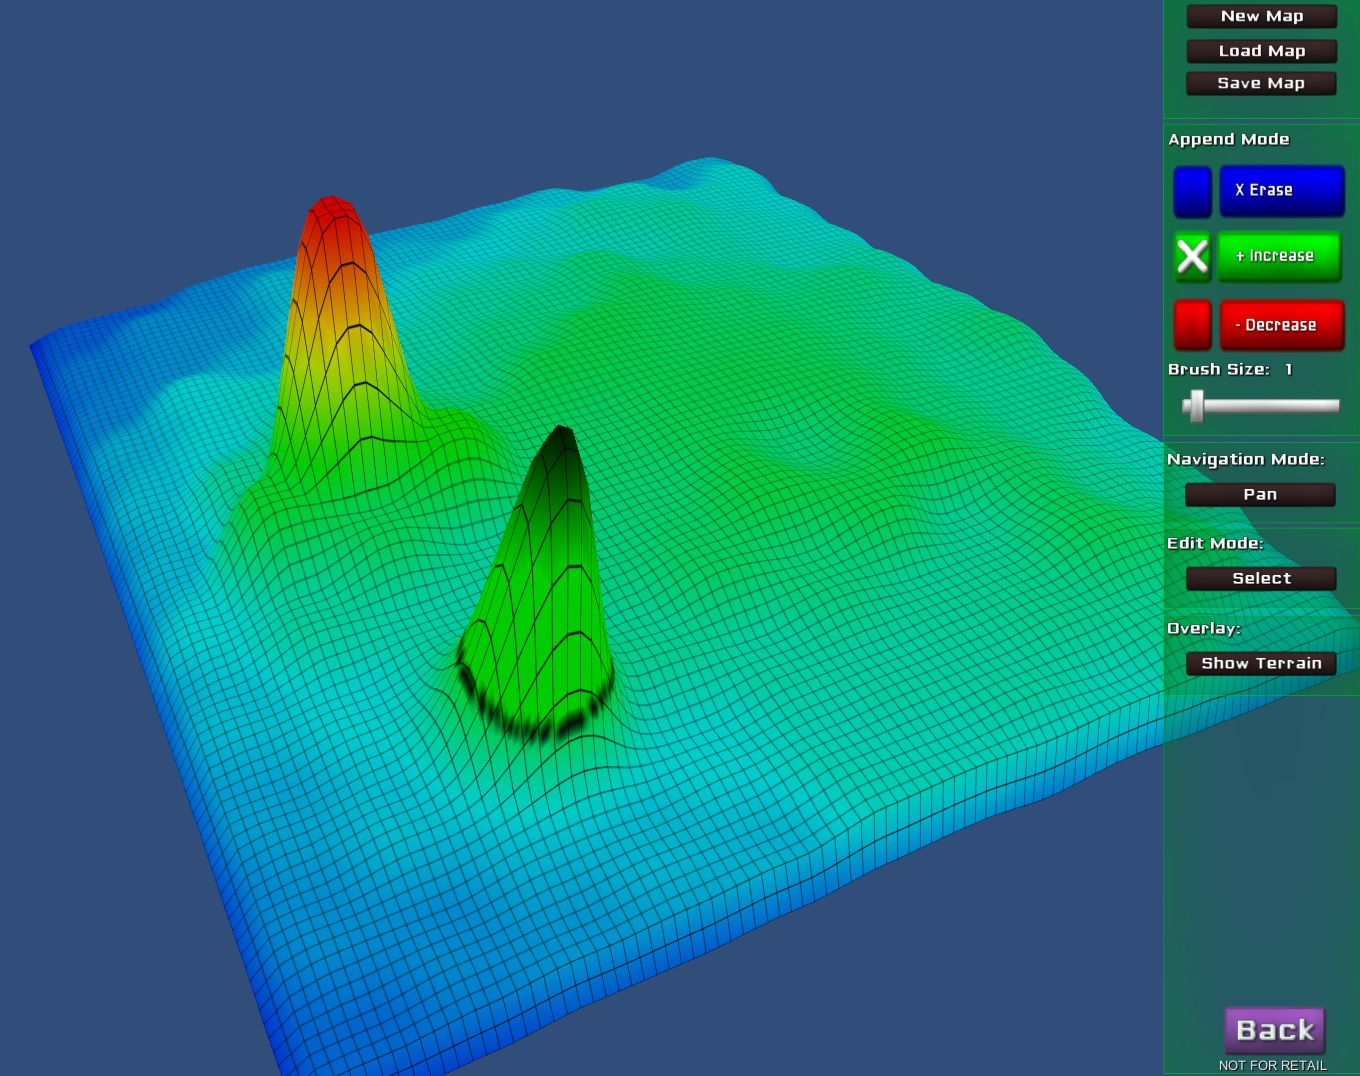
\includegraphics[width=6in]{DistEdit005.JPG}
\caption{To be added}
\label{DistEdit005}
\end{figure}



Users will modify the distribution by making mouse gestures over a 2D representation of the distribution map where colors are used to represent the probability density (e.g., red for high probability hills and blue for low probability plains/valleys). The searchers can switch to a 3D view (read-only) for a better view of the distribution surface. The modified probability distribution can be used later to prioritize tasks and plan UAV paths. By marking an area as a high priority area, the searchers can indirectly manipulate the UAV to search the area before other areas without the need to manually specify waypoints. 



